\documentclass[gra_conf.tex]{subfiles}
 
\begin{document}

En los diferentes modos que posee el brazo, se puede manejar de una manera 
más eficiente a través de una máquinas de estado, para empezar en la fig.1 
se representa esta lógica con el diagrama de estado.

\begin{figure}[h]
  \centering
  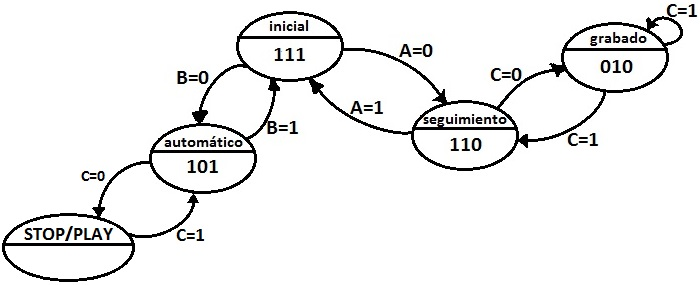
\includegraphics[width=0.4\textwidth]{../img/machine.jpg}
  \caption{Muestra de maquina de estados}
  \label{state_machine_lol}
\end{figure}

Básicamente el brazo posee 4 operaciones fundamentales, mencionados a 
continuación.

\begin{itemize}
\item Inicial: Estado en reposo del brazo robótico.

\item Seguimiento: Mediante el brazo a escala, el brazo robótico reproduce 
los movimientos. 

\item Grabado: Obtención de posiciones, las cuales serán guardadas en la 
memoria.

\item Automático: Reproducción de movimiento, a través de las coordenadas.

\item STOP/PLAY: Detener o reanudar el proceso de automatización.

\end{itemize}

Estos estados se definen gracias a las lecturas digitales,denominadas para 
el presente caso como A, B y C. Para variar las lecturas digitales se 
recurre al uso de un pulsador y un switch triple.

\begin{figure}[h]
\centering
  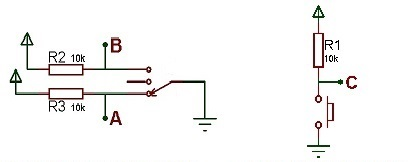
\includegraphics[width=2.5in]{../img/final_abc.jpg}
  \begin{center}
  \caption{ (a) Lectura digital de A y B  (b) Lectura digital de C}
  \end{center}
  \label{final_abc}
\end{figure}


En la Fig. \ref{final_abc}.a se aprecian dos pulsadores en pull-up
y Fig. \ref{final_abc}.b, se aprecia un pull-up, de los posibles
resultados de estas lecturas, se consiguen claramente 6 estados,
donde cada estado está definida por una operación. 

Por motivos de operaciones básicas solo se reduce a 4 estados, estas 
operaciones son mostradas en la tabla \ref{table:states}.

\begin{table}
  \caption{Tabla de e}
  \label{table:states}
  \begin{center}
    \begin{tabular}{|c|c|c|c|}
      \hline
      C & B & A & Operación \\
      \hline
      0 & 1 & 0 & grabado \\
      \hline
      1 & 1 & 0 & seguimiento \\
      \hline
      1 & 0 & 1 & automático\\
      \hline
      1 & 1 & 1 & inicial\\
      \hline
    \end{tabular}
  \end{center}
\end{table}
   
\begin{figure}[h]
  \centering
  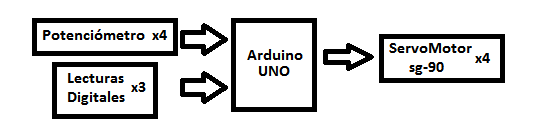
\includegraphics[width=0.4\textwidth]{../img/Interfaz.png}
  \caption{Interfaz de funcionamiento}
  \label{state_abc}
\end{figure}

El Arduino toma como entrada 4 valores analógicos de los potenciómetros
para el control de los ServoMotores, y 3 valores digitales, cuyas
permutaciones indican diferentes estados.

\end{document}

%\documentclass[main_conf.tex]{subfiles}
% 
%\begin{document}


%\end{document}